\documentclass[11pt, oneside]{article} 
\usepackage{geometry}
\geometry{letterpaper} 
\usepackage{graphicx}
	
\usepackage{amssymb}
\usepackage{amsmath}
\usepackage{parskip}
\usepackage{color}
\usepackage{hyperref}

\graphicspath{{/Users/telliott/Github/figures/}}
% \begin{center} 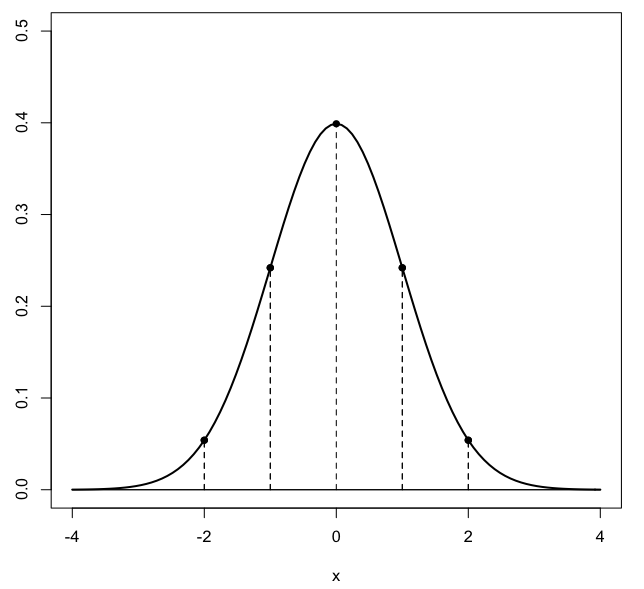
\includegraphics [scale=0.4] {gauss3.png} \end{center}

\title{Triangle inequality}
\date{}

\begin{document}
\maketitle
\Large

Here we prove the theorem known as the \textbf{triangle inequality}, which is then used in proving numerous additional theorems in analysis.  It is connected to the idea of absolute value.

\subsection*{Absolute value}

The absolute value function (abs in Python) is typeset as $|x|$ and defined as follows:
\[
f(x) = |x| = 
\begin{cases}
\ \ 0, \ \ \ x = 0 \\
\ \ x, \ \ \ x > 0 \\
-x, \ \ \ x < 0
\end{cases}
\]

This could be simplified by combining the first two cases into one statement:  $|x| = x$ for $x \ge 0$.  But in what follows we will usually consider the three cases separately.

\subsection*{triangle inequality}

We will prove this theorem 
\[ |x + y| \le |x| + |y| \] 

This inequality holds regardless of the signs of $x$ and $y$.

\subsection*{Aside on geometry}
The triangle inequality is named after the version from geometry.  

When considering the lengths of the sides of a triangle (or the distances between three points in the plane), the lengths of any two sides added together are greater than the length of the third side.  Equality is found for the limiting case when the triangle collapses.

\begin{center} 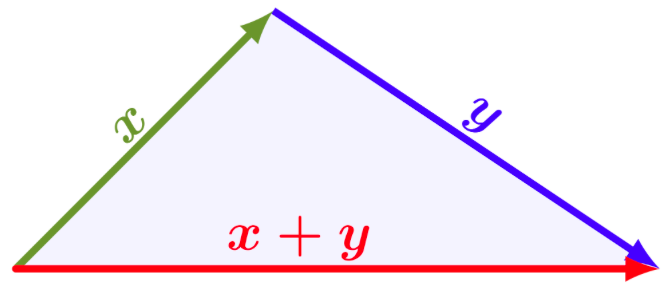
\includegraphics [scale=0.3] {triangle_inequality.png} \end{center}

Euclid claims that the shortest distance between any two points is a straight line (in this figure from the web, $\mathbf{x + y}$ refers to the \emph{vector sum} of $\mathbf{x}$ and $\mathbf{y}$).

For the real number line, consider any two values $a$ and $b$.  
\begin{center} \includegraphics [scale=0.4] {triangle_inequality_2.png} \end{center}

These are \emph{signed} values so there are a number of cases, namely $a > 0$, $a = 0$ and $a < 0$, and the same for $b$.  That's a total of six.  

The length of an arrow is a separate concept, where length is \emph{always non-negative}.  The absolute value function is a way of talking about length.

So, quite clearly, if $a$ and $b$ are both non-zero and have the same sign (left panel), the length of their sum $|a + b|$ is equal to the sum of the lengths $|a| + |b|$.  This is also true if one or both is equal to zero.
\[ |a + b| = |a| + |b| \]

However, when the signs are different (both lengths non-zero), then the length of the sum is always smaller than the larger length, and certainly
\[ |a + b| < |a| + |b| \]

These cases are combined to form the inequality:
\[ |a + b| \le |a| + |b| \]

\subsection*{theorem}

One way to prove the theorem
\[ |x + y| \le |x| + |y| \] 
is to go through cases.  

It seems like it should be pretty straightforward, but one can quickly get tied up in knots.

In the statement (and the definition of $|x|$), we allow $x < 0$, and in that case the definition says $|x| = - x$.  This becomes confusing because $- x$ is greater than zero, so we need to be explicit.  The first cases, where one or both of $x$ and $y$ is zero, are trivial.

One is positive and one is zero.  Without loss of generality:

$\bullet$ \ $x > 0, y = 0$

By the definition, $|x| + |y| = x + 0 = x$ and since $x + y > 0$,  $|x + y| = x + y = x + 0 = x$.  We have equality:  $|x| + |y| = |x + y|$.

One is negative and one is zero.  Without loss of generality:

$\bullet$ \ $x < 0, y = 0$

Then $|x| + |y| = -x + 0 = -x $ and since $x + y < 0$,  $|x + y| = -(x + y)  = -(x + 0) = - x$.  Equality again.

Both are zero:

$\bullet$ \ $x = 0, y = 0$

Then $|x| + |y| = 0 + 0 = 0 = |x + y|$.

Now for all the non-zero cases:

$\bullet$ \ $x > 0, y > 0$

We have that $x + y > 0$ so by the definition:
\[ x + y = |x + y| \]
and since individually $x > 0, y > 0$
\[ x + y = |x| + |y| \]

$\bullet$ \ $x < 0, y < 0$

We have that $x + y < 0$ so by the definition:
\[ |x + y| = - (x + y) \]
and individually
\[ |x| + |y| = - x - y = - (x + y) \]

Inequality comes when the values are non-zero and different.  This is the part that's a little bit tricky.

$\bullet$ \ $x > 0, y < 0$ and neither is equal to zero.  So by this main premise:  $|x| = x$ and $|y| = - y$.  Break this up into sub-cases.  Remember that for a non-zero value $x$, always $|x| > 0$.

$\circ$ \ $|x| > |y|$

By the sub-premise, we have that $x > -y$ so $x + y > 0$, and then, by the definition:
\[ |x + y| = x + y \]
Starting with $y < 0$, we add a positive quantity $x > 0$ to both sides:
\[ x + y < x \]
but
\[ x = |x| < |x| + |y| \]
so
\[ |x + y| <  |x| + |y| \]

$\circ$ \ $|x| = |y|$

By the sub-premise, and $|x| = x$ and $|y| = - y$, we have that $x + y = 0$ so
\[ |x + y| = 0 \]
And then
\[ x + y = 0 < x = |x| < |x| + |y| \]
so
\[ |x + y| <  |x| + |y| \]

$\circ$ \ $|x| < |y|$

By the sub-premise, we have that $x + y < 0$ so
\[ |x + y| = -(x + y) = - x - y \]
Now, $x > 0$ and $y < 0$ so
\[ |x| = x > -x \]
\[ |y| = -y \]
Plugging in
\[ |x + y| = -(x + y) = - x - y < |x| + |y| \]

Therefore, in every case
\[ |x + y| \le |x| + |y| \]

Almost three pages for the simple proof!

\section{Interval with midpoint}

For a formal approach (especially helpful for the case of different signs), we follow Apostol.  We consider a preliminary theorem first, which is another result frequently used in analysis.

Consider an open interval whose endpoints are equidistant from a central point $p$, where the distance to the boundary is $a$ (as a \emph{distance}, certainly $a > 0$), and  $x$ is contained somewhere in the open interval $(p-a,p+a)$

\begin{center} 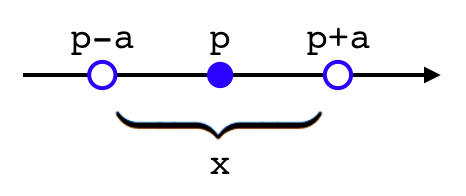
\includegraphics [scale=0.4] {neighborhood2.png} \end{center}

We can translate this picture to algebra as
\[ p - a < x < p + a \]
Adding $-p$ to each term
\[ -a < x - p < a \]

The preliminary theorem states that the above is true if and only if
\[ |x - p| < a  \]
We should read the last statement as saying that the distance between $x$ and $p$ is less than $a$.

Taking the statements above
\[ |x - p| \le a \iff -a \le x - p \le a \]
and rewriting $x -p$ as just $x$ we obtain:  
\[ |x| \le a \iff -a \le x \le a \]
This is the statement we will prove.

\subsubsection*{preliminary preliminary theorem}

There is actually another theorem that comes before the preliminary theorem.
\[ -|x| \le x \le |x| \]

\subsubsection*{proof}

We just do this one by cases.

$\circ$   If $x \ge 0$ then $x = |x|$ and $-|x| < 0$ so $x \ge -|x|$.

$\circ$   If $x < 0$, then $|x|=-x$ and $x = -|x|$ and also $|x| \ge 0$ so $x < |x|$.

$\circ$   If $x = 0$ we have equality.

\subsection*{preliminary theorem}

\[ |x| \le a \iff -a \le x \le a \]

\subsection*{proof}
Let $a$ be a constant real number $a > 0$ and the starting proposition is
\[ |x| \le a \]
Add the expression $-a - |x|$ to both sides to obtain
\[ -a \le - |x| \]

From the preliminary preliminary theorem we obtain
\[ -|x| \le x \le |x| \]

We combine all three parts:
\[ -a \le -|x| \le x \le |x| \le a \]
which simplifies to
\[ -a \le x \le a \]
This completes the forward proof.

To prove the converse, we are assuming that
\[ x \le a \]
and
\[ - a \le x \]
Now if $x \ge 0$ we have $|x| = x$ so
\[ |x| = x \le a \]
On the other hand for $x < 0$, we start with the first part
\[ -a \le x \]
Add $a - x$ to both sides
\[ -x \le a \]
and since $x < 0$, $|x| = -x$ and we have 
\[ |x| =  -x \le a \]
In both cases we have \[ |x| \le a \]
and this completes the proof.

$\square$

\subsection*{continuity example}

\begin{center} 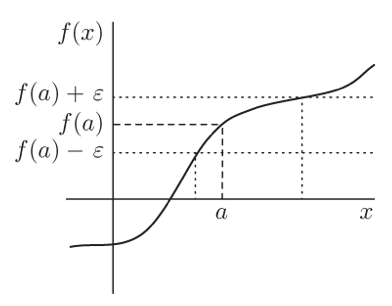
\includegraphics [scale=0.6] {continuity3.png} \end{center}

As motivation for this whole topic, in the definition of \textbf{continuity} of a function $f(x)$ at a point $a$, we play the epsilon-delta game.  Choose an \emph{arbitrary} positive real number $\epsilon > 0$.  

Then we say, $f$ is continuous at $a$ if and only if we can find $\delta$ such that 
\[ |x - a| < \delta \Rightarrow |f(x) - f(a)| < \epsilon \]

If the distance (or difference) between $x$ and $a$ is less than $\delta$, then it follows that the difference $|f(x) - f(a)|$ is less than $\epsilon$.

The last statement is exactly the same as
\[ -\epsilon < f(x) - f(a) < \epsilon \]

The advantage of this formulation is that there are no absolute value signs so we can rearrange the above to give:

\[ f(a) -\epsilon < f(x) < f(a) + \epsilon \]

We will see multiple examples of this in real analysis.

\subsection*{alternative proof (by examining cases)}
The statement
\[ -a < x - p < a \Rightarrow  |x - p| < a  \]
may be proved informally by going exhaustively through the cases, as follows.

(1) If $x = p$ then $x - p = 0 < a$ and $0 > -a$; 

(2) If $x > p$, then $x - p > 0$ and so 
\[ |x - p| = x - p \]
Then
\[ x - p < a \] 
implies 
\[ |x - p| = x - p < a \]
and since the absolute value is positive it is certainly $> -a$.

(3) If $x < p$ then $x - p < 0$ so
\[ |x - p| = -(x-p) = p - x \]
Then the first part of the assumption is
\[ -a < x - p \] 
Add $a + p - x$ to both sides
\[ p - x < a \]
which implies
\[ |x - p| = p - x < a \]
and again the absolute value is positive so it is certainly $> -a$.

This proves the theorem.

$\square$

\section{Triangle inequality}

Let us change the notation of the previous theorem so we can reuse the variable $x$ in the next part:
\[ | \phi | \le a \iff -a \le \phi \le a \]

Now start by considering
\[ - |x| \le x \le |x| \]
Now add two such inequalities 
\[ - \ [ \ |x| +  |y| \ ] \  \le x + y \le  |x| + |y|  \]

Recall the theorem we just proved with its new notation and focus on the right-hand side
\[  -a \le \phi \le a \]
Equate $a$ with $|x| + |y|$ and $\phi$ with $x + y$.  

Then the expression that we had above by adding two inequalities
\[ - \ [ \ |x| +  |y| \ ] \  \le x + y \le  |x| + |y|  \]
can be seen as equivalent to the right-hand side from the theorem.  
\[  -a \le \phi \le a \]

Therefore, the left-hand side must also be true, namely
\[ |\phi| \le a \]
\[ |x + y| \le  |x| +  |y| \]
This proves the triangle inequality.

$\square$


We next consider a related theorem and some corollaries:
\[ |x - y| \ge |x| + |y| \]
\[ |xy| = |x| \ |y| \]
\[ |x - y| = |y - x| \]
\[ |x - y| \le |x - z| + |z - y| \]

\section{Additional theorems}
The first one is trivial:  the triangle inequality applies no matter if $y$ is negative.  So if we think of $y > 0$ and then add a minus sign to it:
\[ |x - y| \ge |x| + |y| \]

\subsection*{multiplication of absolute values}
\[ |xy| = |x| \ |y| \]

Obviously true for equal signs or one of $x,y$ equal to zero.  For different signs ($m,n > 0; \ \ x = -m, y = n$):
\[ |xy| = |(-m)n| = |-mn| = mn = |-m| \ |n| = |x| \ |y| \]
$\square$

\subsection*{theorem:  change of sign}
\[ |x - y| = |y - x| \]

\subsection*{easy proof}

Regardless of whether $x \ge 0$ or $x < 0$, by the definition of absolute value
\[ |x| = |-x| \]

Substitute $x - y$ for $x$
\[ |x - y| = |-(x - y)| = |y - x| \]

\subsection*{first proof}
Suppose that $m,n > 0$ and $x = m, y =-n$.

$\circ$  $m > n$ so $m - n = p > 0$
\[ |x - y| = |m - n| = |p| = p \]
\[ |y - x| = |n - m| = |-p| = p \]
so
\[ |x - y| = |y - x| \]
Having $n > m$ does not change the argument

$\circ$  $n > m$ so $m - n = -p < 0$
\[ |x - y| = |m - n| = |-p| = p \]
\[ |y - x| = |n - m| = |p| = p \]

\subsection*{theorem:  third variable}
\[ |x - z|  \le |x - y| + |z - y| \]

\subsection*{proof}
Start with the triangle inequality
\[ |x + y| \le |x| + |y| \]

Suppose that what is meant is $x,y > 0$.  It doesn't matter since the triangle theorem holds regardless of the signs of the two terms.

Replace $x$ by $x-y$ and $y$ by $y-z$ 
\[ |x-y + y-z| \le |x-y| + |y-z| \]
\[ |x - z|  \le |x - y| + |z - y| \]

We can substitute letters if you prefer something different
\[ |x - y|  \le |x - z| + |y - z| \]

We can switch the order for any term by the first corollary above.  So
\[ |x - y|  \le |x - z| + |y - z| \]

goes to
\[ |x - y|  \le |x - z| + |z - y| \]

\subsection*{theorem:  subtraction}
\[  |x - y| \ge |x| - |y|  \]

\subsection*{proof}
\[ |x + y| \le |x| + |y| \]

Replace $x$ by $x - y$
\[ |x| \le |x - y| + |y| \]
\[ |x - y| \ge |x| - |y| \]

\subsection*{Summary}
\[ |x + y| \le  |x| +  |y| \]
\[ |xy| = |x| \ |y| \]
\[ | x - z | \le | x - y | + | y - z | \]
\[ |x - y| \ge |x| - |y| \]

\section{Extension}

\subsection*{theorem}

\[ |x_1 + x_2 + \dots + x_n| \le |x_1| + |x_2| + \dots + |x_n| \]

\subsection*{proof}

By induction.  Let $x$ be equal to the sum of all the terms before the last one.
\[ x = x_1 + x_2 + \dots + x_{n-1} \]

We may assume that
\[ |x| \le  |x_1| + |x_2| + \dots + |x_{n-1}| \] 

By the triangle inequality
\[ |x + x_n| \le |x| + |x_n| \]
But using the assumption we can substitute for $|x|$ and write
\[ |x + x_n| \le |x_1| + |x_2| + \dots + |x_{n-1}| + |x_n| \]
So
\[ |x_1 + x_2 + \dots + x_n| \le |x_1| + |x_2| + \dots + |x_n| \]

$\square$

\subsection*{theorem}
\[ | \ \int_0^1 f(x) \ dx \ | \le \int_0^1 |f(x)| \ dx \]
We won't prove this one, but the analogy with the previous result is pretty clear.


\end{document}